\section{Software correlator}\label{sec:vlbi}
If the data in an {\it e}-VLBI experiment can be streamed over the
internet to JIVE, it can also be sent to another correlator. Within
\scarie, we are investigating the possibilities of a next generation
correlator using a computing Grid. The advantages of a software
correlator over a new dedicated hardware correlator lie in its
flexibility and accuracy. The software correlator can be tuned for
special experiments. The main advantage of a dedicated hardware
correlator is the greater performance. The advance of general purpose
computing is making software correlation a cost-effective solution for
a range of applications. A similar approach is presented in
\cite{deller-2007}.

The flexibility of its architecture allows the software correlator to
change with the needs of researchers. In fact, the first version of
the software correlator was developed to track the Huygens spacecraft
during its descent through the atmosphere of Saturn's moon Titan. Due
to the nature of this experiment, special requirements are put on the
correlator, which the current hardware correlator is not able to
provide.  Moreover, we expect that the costs of developing a software
correlator are much lower than the costs for a hardware correlator.

The correlation is done by splitting the signal in time slices that
are processed in parallel (see Figure~\ref{fig:netw_corr}). The signal
from a telescope is received by a single so-called input node.  The
input node sends slices of data to an available correlator node. The
correlator node receives data from all telescopes for a certain time
slice and performs the correlation. The size of the output of the
correlation is much smaller than the input size and can be collected
and stored by a single output node.  There is a single manager node
that assigns data to available computing nodes.

The correlation is not computationally expensive, in the sense that it
requires only few operations per transferred bytes. However, due to
the high data rates, the absolute number of clock cycles required by
the application is still extremely high. Moreover, the problem is
quadratic in the number of telescopes participating in the experiment
since it is linear in the number of channel pairs that have to be
correlated. The huge need for networking and computing power makes a
computing Grid an ideal platform for this application.


\begin{figure}
  \centering
  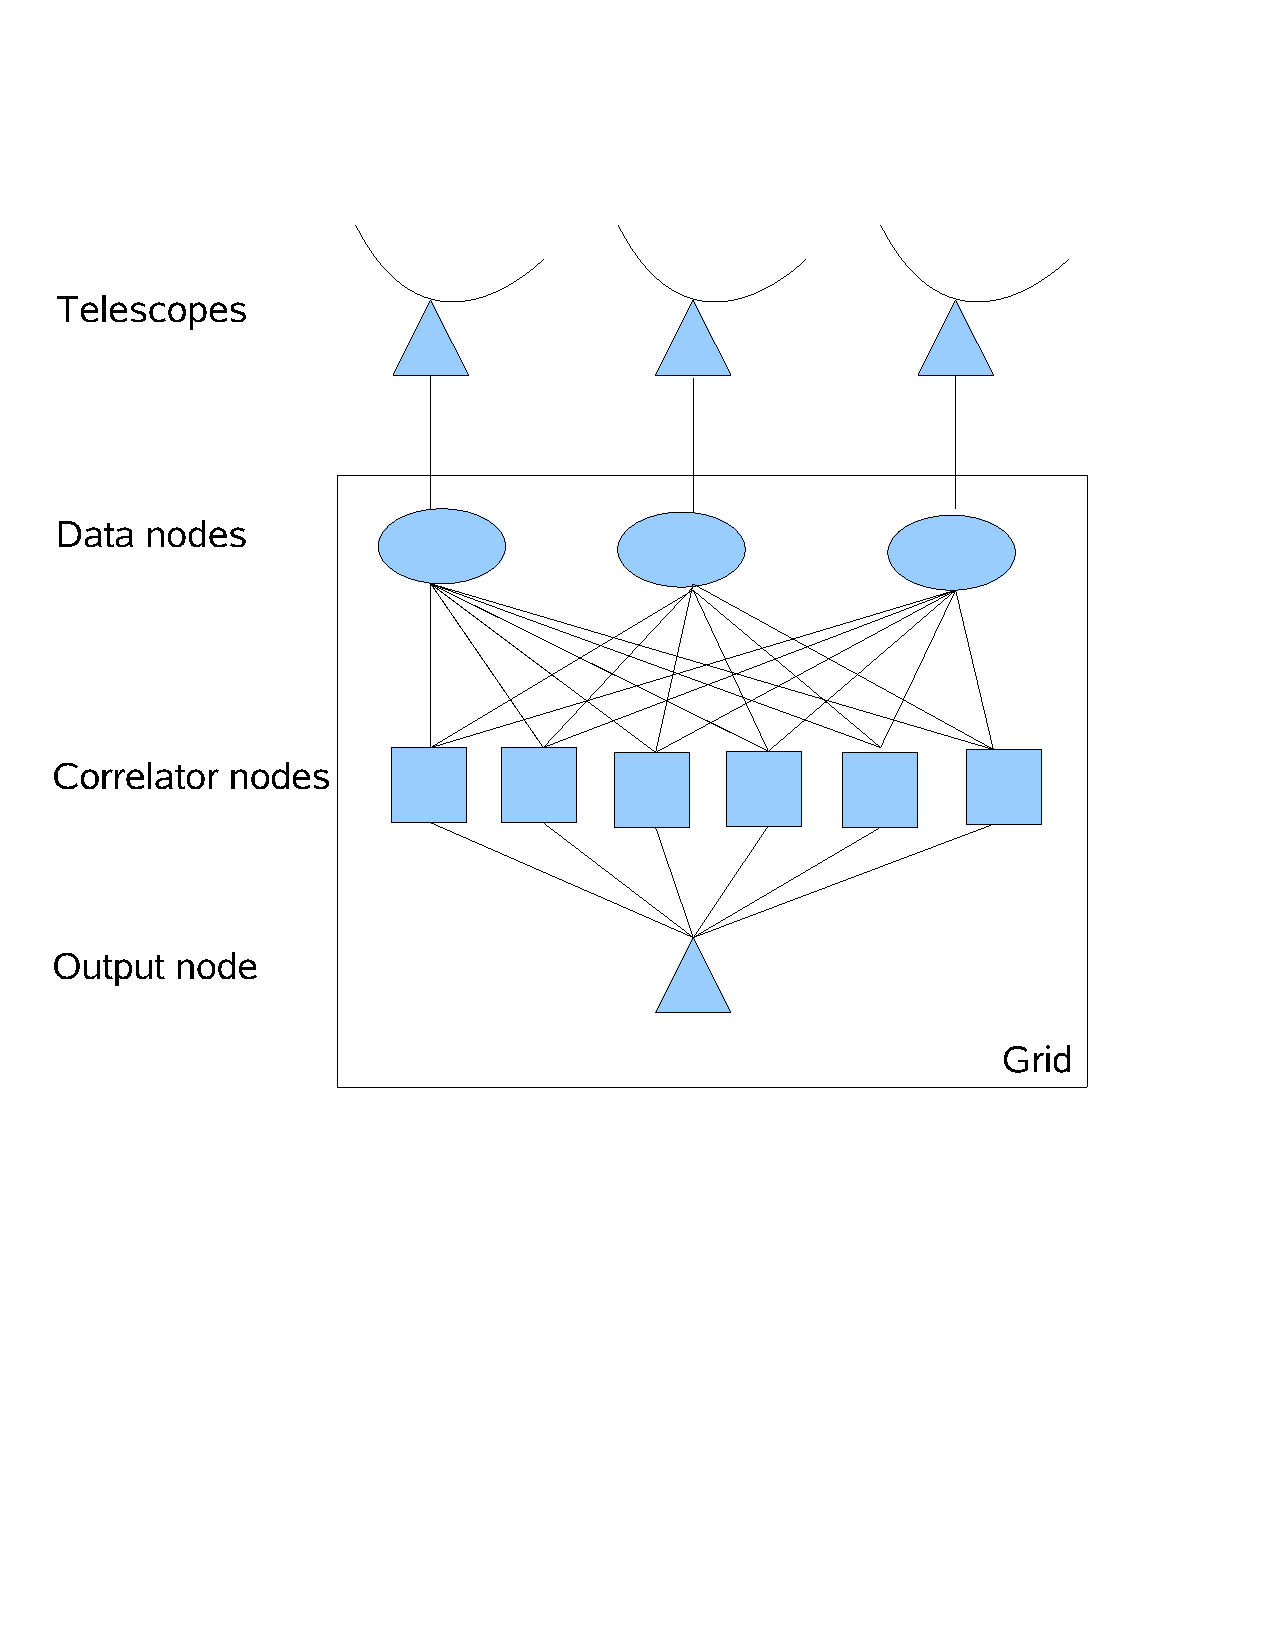
\includegraphics[width=.45\textwidth]
    {img/NetworkConnections}
    \caption{Outline of the network connections between different
      components in the software correlator.}
  \label{fig:netw_corr}
\end{figure}


\subsection{Design}
The software correlator is written in \verb~C++~ and uses several
standard libraries like \verb~fftw~ \cite{FFTW05}, \verb~mpich~
\cite{Gropp:1996:HPI}, , \verb~GSL~ \cite{GSL} and the
standard template library.

At initialization, each node is assigned a role: input node, correlator
node, output node or manager node. The node then creates a number of
controllers that manage different tasks of the node. 

\paragraph{Input node}
The input node receives the data from a single data stream and
\marginpar{NGHK: Continue}. It then connects the two using a buffer.
The input node will receive a message from the manager node specifying
how to obtain the input: from file or over the network using one of
various types of transfer protocols. It will also receive messages
containing a start and stop time and the correlator node to send the
data to.

\paragraph{Correlator node}
A correlator node will initialize the correlation process and connect
to the output node. It can receive messages from a input node asking to
open an input connection and from the manager node to process a
time slice. After the slice is processed the node will send a message
to the manager node saying it is available for a next job.

\paragraph{Output node}
The output node will receive a message from the manager node where
to store the data, and it allows connections from the correlator node to
be opened. The node sorts the received data from the correlator nodes
and stores it for further processing. The output node has to make the
received data available to the user, and it should be archived in a
proper way.

\paragraph{Manager node}
The manager node is the most complicated node in the software
correlator. It sends messages to initialize the other nodes and tells
them how to connect to each other. After the initialization, it
maintains a list of available correlator nodes and delegates time
slices to available correlator nodes. General error messages can also
be sent from any node to the manager node.

The interface to the user will communicate with the manager node to
send commands to the correlator and obtain status information from the
correlator. The user interface will be based on Virtual lab.

\subsection{Network connections}
Since correlation is mainly a networking problem, testing and
optimizing the data flows is of vital importance for the performance
of the software correlator. We distinguish two types of data flows:
containing control messages and the signals from the telescopes. 

\paragraph{Control messages}
The control messages are sent between different nodes to regulate the
correlation. They form a low bandwidth stream and MPI is used to send
these messages. The network is mainly star shaped around the control
node, but there are some connections during the initialization between
input nodes and the correlator nodes and between correlator nodes and
the output node. Since the messages control the correlator, the
delivery of the messages has to be guaranteed. For the analysis of the
network throughput these messages are of no importance.

\paragraph{Signal of the telescopes}
The signal from the telescopes requires far more bandwidth than the
control messages. The constant throughput for these connections is
very important as we are dealing with real time data. Some packet loss
is even acceptable if a data stream at a constant rate can then be
maintained. The connections for these data streams are set up to be
exchangeable such that it is possible to test different network
protocols like TCP (using jumbo frames), or protocols used for
streaming media. The network consists of three layers: from the
telescopes to the data nodes, then to the correlator nodes and finally
to the output node, as is shown in
Figure~\ref{fig:netw_corr}.\marginpar{NGHK: mention StarPlane}



%%% Local Variables:
%%% mode: latex
%%% TeX-master: "Ingrid"
%%% End:
